\chapter{Parcial 1}


\section{Sobre esta guía}\index{Sobre la guía}

La siguiente guía tiene como objetivo presentar de manera sistemática los contenidos teórico práctico de la asignatura \textbf{Programación de aplicaciones web} en base al plan de carrera del Instituto Tecnológico Benito Juárez en su rediseño del año 2016 para Desarrollo de Software.

\begin{center}
	Datos generales de la asignatura\\
		\begin{tabular}{ |c|c| } 
			\hline
			Nombre de la asignatura: & Programación Aplicaciones Web \\
			\hline
			Campo de formación: & Adaptación tecnológica e innovación \\ 
			\hline
			Unidad de organización curricular: & Formación técnica profesional \\
			\hline
			Número de período académico: & 4 \\
			\hline
			Número de horas de la asignatura: & 122 \\
			\hline
			Número de horas por cada componente: & 
			\begin{tabular}{c}
				Docencia: 60\\
				Prácticas de aprendizaje: 24 \\ 
				Aprendizaje autónomo: 38 \\
			\end{tabular} \\
			\hline
			Docente: & Freddy Heredia: \textbf{\texttt{fheredia@yavirac.edu.ec}}\\
			\hline
		\end{tabular}
\end{center}


\section{Lo que aprenderás}

\section{El origen} \index{El origen}

\cite{sl}Aunque los inicios de Internet se remontan a los años setenta, no ha sido hasta los años noventa cuando, gracias a la Web, se ha extendido su uso por todo el mundo. En pocos años la Web ha evolucionado enormemente: se ha pasado de páginas sencillas, con pocas imágenes y contenidos estáticos a páginas complejas con contenidos dinámicos que provienen de bases de datos, lo que permite la creación de "aplicaciones web".
\\\\
\cite{sl}Internet y la Web han incluido enormemente tanto en el mundo de la informática
como en la sociedad en general. Si nos centramos en la Web, en poco menos de 10
años ha transformado los sistemas informáticos: ha roto las barreras físicas (debido a
la distancia), económicas y lógicas (debido al empleo de distintos sistemas operativos,
protocolos, etc.) y ha abierto todo un abanico de nuevas posibilidades. Una de las áreas
que más expansión está teniendo en la Web en los últimos años son las aplicaciones
web.
\\\\
\cite{sl}Las aplicaciones web permiten la generación automática de contenido, la creación
de páginas personalizadas según el perfil del usuario o el desarrollo del comercio electrónico. Además, una aplicación web permite interactuar con los sistemas informáticos de gestión de una empresa, como puede ser gestión de clientes, contabilidad o
inventario, a través de una página web.
\\\\
\cite{sl}De forma breve, una aplicación web se puede definir como una aplicación en la cual el usuario por medio de un navegador realiza peticiones a una aplicación remota accesible a través de internet (o a través de una Intranet) y que recibe una respuesta que se muestra en el propio navegador.

\begin{remark}
	\url{https://rua.ua.es/dspace/bitstream/10045/16995/1/sergio_lujan-programacion_de_aplicaciones_web.pdf}
\end{remark}


\subsection{Protocolos de internet} \index{Protocolos de internet}
El éxito de Internet se basa mucho en el empleo de TCP/IP, el conjunto de protocolos de comunicación que permiten el intercambio de información de forma independiente de los sistemas en que ésta se encuentra almacenada. TCP/IP constituye
la solución problema de heterogeneidad de los sistemas informáticos. El 1 de enero de
1983, TCP/IP se estableció como el protocolo estándar de comunicación en Internet.\\
El conjunto de protocolos TCP/IP, también llamado la pila de protocolos
TCP/IP, incluye una serie de protocolos que se encuentran en el nivel 7 o de aplicación de la arquitectura Open System Interconnection (OSI) y que proporcionan una
serie de servicios.\\
Como un mismo ordenador puede atender varios servicios, cada servicio se identifica con un número llamado puerto. Por tanto, a cada protocolo le corresponde un
número de puerto. Los protocolos que se encuentran estandarizados poseen un puerto
reservado que no puede emplear ningún otro protocolo.

En el siguiente cuadro se muestran los protocolos del nivel 7 más comunes de Internet
junto con el número de puerto que emplean.

\cite{osi}En la siguiente imagen se muestran las capas del modelo OSI:

\begin{figure}[H]
	\center
	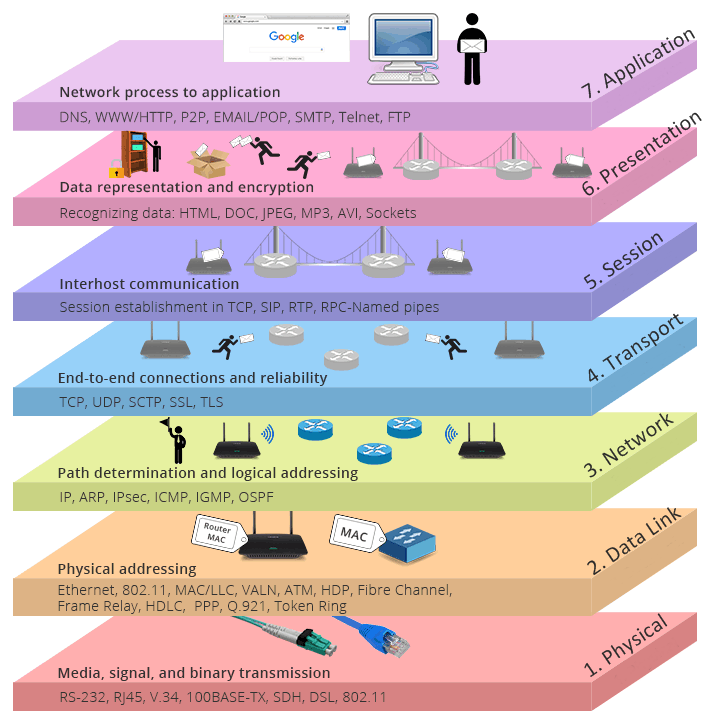
\includegraphics[width=0.7\textwidth]{osi.png}
	\caption{Modelo OSI}
	\label{fig:super}
\end{figure}

\begin{remark}
Véa el siguiente vídeo: Guerreros de la red \\
\url{https://youtu.be/1c2U1R8XXvA}
\end{remark}
\section{Arquitecturas cliente/servidor} \index{Arquitectura cliente/servidor}

\cite{sl}Las aplicaciones web son un tipo especial de aplicaciones cliente/servidor. Antes de
aprender a programar aplicaciones web conviene conocer las características básicas de las
arquitecturas cliente/servidor.

Cliente/servidor es una arquitectura de red
en la que cada ordenador o proceso en
la red es cliente o servidor
. Normalmente, los servidores son ordenadores potentes
dedicados a gestionar unidades de disco (servidor de ficheros), impresoras (servidor de impresoras), tráco de red (servidor de red), datos (servidor de bases de datos) o
incluso aplicaciones (servidor de aplicaciones), mientras que los clientes son máquinas
menos potentes y usan los recursos que ofrecen los servidores.

Esta arquitectura implica la existencia de una relación entre procesos que solicitan
servicios (clientes) y procesos que responden a estos servicios (servidores). Estos
dos tipos de procesos pueden ejecutarse en el mismo procesador o en distintos.

La arquitectura cliente/servidor permite la creación de aplicaciones distribuidas.
La principal ventaja de esta arquitectura es que facilita la separación de las funciones
según su servicio, permitiendo situar cada función en la plataforma más adecuada
para su ejecución. Además, también presenta las siguientes ventajas:
\begin{itemize}
	\item Las redes de ordenadores permiten que múltiples procesadores puedan ejecutar
	partes distribuidas de una misma aplicación, logrando concurrencia de procesos.
	\item Existe la posibilidad de migrar aplicaciones de un procesador a otro con modificaciones mínimas en los programas.
	\item Se obtiene una escalabilidad de la aplicación. Permite la ampliación horizontal
	o vertical de las aplicaciones. La \textbf{escalabilidad horizontal} se refiere a la capacidad de añadir o suprimir estaciones de trabajo que hagan uso de la aplicación
	(clientes), sin que afecte sustancialmente al rendimiento general, La \textbf{escalabilidad vertical} se refiere a la capacidad de migrar hacia servidores
	de mayor capacidad o velocidad, o de un tipo distinto de arquitectura sin que
	afecte a los clientes.
	\item Posibilita el acceso a los datos independientemente de donde se encuentre el
usuario.
\end{itemize}	

\subsection{Separación de funciones}\index{Separación de funciones}

La arquitectura cliente/servidor nos permite la separación de funciones en tres
niveles:

\begin{itemize}
\item \textbf{Lógica de presentación}. Se encarga de la entrada y salida de la aplicación con
el usuario. Sus principales tareas son: obtener información del usuario, enviar la
información del usuario a la lógica de negocio para su procesamiento, recibir los
resultados del procesamiento de la lógica de negocio y presentar estos resultados
al usuario.

\item \textbf{Lógica de negocio (o aplicación).} Se encarga de gestionar los datos a nivel
de procesamiento. Actúa de puente entre el usuario y los datos. Sus principales
tareas son: recibir la entrada del nivel de presentación, interactuar con la lógica
de datos para ejecutar las reglas de negocio (business rules) que tiene que cumplir la aplicación (facturación, cálculo de nóminas, control de inventario, etc.) y
enviar el resultado del procesamiento al nivel de presentación.


\item \textbf{Lógica de datos.} Se encarga de gestionar los datos a nivel de almacenamiento.
Sus principales tareas son: almacenar los datos, recuperar los datos, mantener
los datos y asegurar la integridad de los datos.
\end{itemize}	

\begin{figure}[H]
	\center
	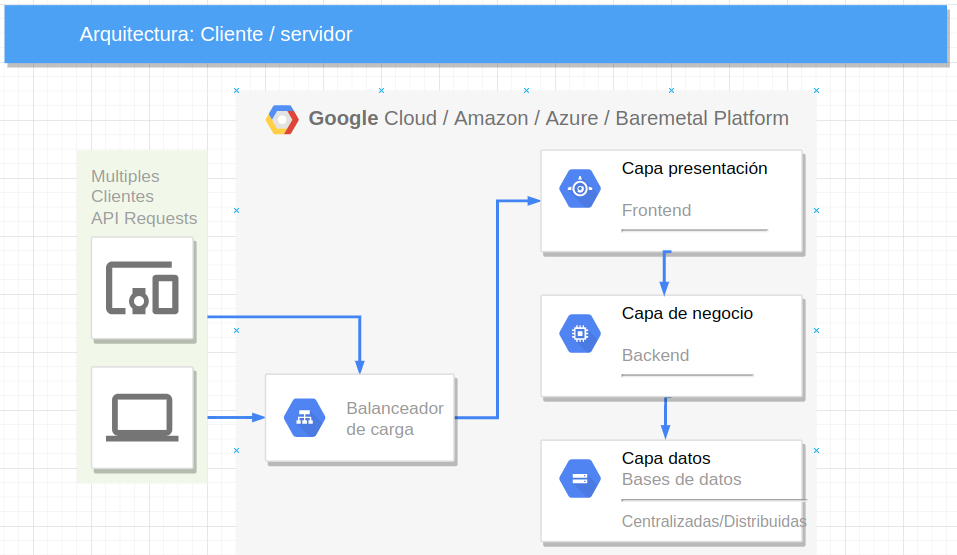
\includegraphics[width=1\textwidth]{arquitectura-cliente-servidor.png}
	\caption{Arquitectura cliente/servidor}
	\label{fig:super}
\end{figure}

\subsection{El cliente}
\cite{mdn}El cliente es cualquier herramienta que actué en representación del usuario para solicitar a
un servidor web el envío de los recursos que desea obtener mediante HTTP. Esta función es realizada en la mayor parte de los casos por un navegador Web. Hay excepciones, como el caso de programas específicamente usados por desarrolladores para desarrollar y depurar sus aplicaciones. 
\\
El navegador es siempre el que inicia una comunicación (petición), y el servidor nunca la comienza (hay algunos mecanismos que permiten esto, pero no son muy habituales).  
\\
Para poder mostrar una página Web, el navegador envía una petición de documento HTML al servidor. Entonces procesa este documento, y envía más peticiones para solicitar scripts, hojas de estilo (CSS), y otros datos que necesite (normalmente vídeos y/o imágenes). El navegador, une todos estos documentos y datos, y compone el resultado final: la página Web. Los scripts, los ejecuta también el navegador, y también pueden generar más peticiones de datos en el tiempo, y el navegador, gestionará y actualizará la página Web en consecuencia. 
\\
Una página Web, es un documento de hipertexto (HTTP), luego habrá partes del texto en la página que puedan ser enlaces (links) que pueden ser activados (normalmente al hacer click sobre ellos) para hacer una petición de una nueva página Web, permitiendo así dirigir su agente de usuario y navegar por la Web. El navegador, traduce esas direcciones en peticiones de HTTP, e interpretara y procesará las respuestas HTTP, para presentar al usuario la página Web que desea.
\\
La parte cliente de las aplicaciones web suele estar formada por el código HTML
que forma la página web más algo de código ejecutable realizado en lenguaje de script
del navegador (JavaScript o VBScript) o mediante pequeños programas (applets) realizados en Java. También se solían emplear plugins que permiten visualizar otros
contenidos multimedia (como Macromedia Flash
), aunque no se encuentran tan extendidos como las tecnologías anteriores y plantean problemas de incompatibilidad
entre distintas plataformas. Por tanto, la misión del cliente web es interpretar las
páginas HTML y los diferentes recursos que contienen (imágenes, sonidos, etc.).
\\
Las tecnologías que se suelen emplear para programar el cliente web son:

\begin{itemize}
	\item HTML
	\item CSS
	\item Javascript
\end{itemize}
\begin{remark}
	Cada tecnología puede tener sus variantes.\\
	WebAssembly es un proyecto prometedor.\\
	Algunas tecnologías ya están en desuso (Applets, Flash entre otras.)
\end{remark}

\subsection{El servidor}
Al otro lado del canal de comunicación, está el servidor, el cual "sirve" los datos que ha pedido el cliente. Un servidor conceptualmente es una unica entidad, aunque puede estar formado por varios elementos, que se reparten la carga de peticiones, (load balancing), u otros programas, que gestionan otros computadores (como cache, bases de datos, servidores de correo electrónico, ...), y que generan parte o todo el documento que ha sido pedido. 
\\
Un servidor no tiene que ser necesariamente un único equipo físico, aunque si que varios servidores pueden estar funcionando en un único computador. En el estándar HTTP/1.1 y Host , pueden incluso compartir la misma dirección de IP.

\subsection{Transferencia de páginas web a través de http}

El proceso completo, desde que el usuario solicita una página, hasta que el cliente
web (navegador) se la muestra con el formato apropiado, es el siguiente:

\begin{enumerate}
	\item El usuario especifica en el cliente web la dirección de la página que desea consultar: el usuario escribe en el navegador la dirección (URL) de la página que
	desea visitar o pulsa un enlace.
	\item El cliente establece una conexión con el servidor web.
	\item El cliente solicita la página o el objeto deseado. 
	\item El servidor envía dicha página u objeto (o, si no existe, devuelve un código de
	error).
	\item Si se trata de una página HTML, el cliente inicia sus labores de interpretación
	de los códigos HTML. Si el cliente web encuentra instrucciones que hacen referencia a otros objetos que se tienen que mostrar con la página (imágenes, sonidos, animaciones multimedia, etc.), establece automáticamente comunicación
	con el servidor web para solicitar dichos objetos.
	\item Se cierra la conexión entre el cliente y el servidor.
	\item Se muestra la página al usuario.
\end{enumerate}

Obsérvese que siempre se libera la conexión, por lo que ésta sólo tiene la duración
correspondiente a la transmisión de la página solicitada. Esto se hace así para no
desperdiciar innecesariamente el ancho de banda de la red mientras el usuario lee la
página recibida.
Cuando el usuario activa un enlace de la página, se establece una nueva conexión
para recibir otra página o elemento multimedia. Por ello, el usuario tiene la sensación
de que está disfrutando de una conexión permanente cuando realmente no es así.
Un detalle importante es que para cada objeto que se transfiere por la red se realiza
una conexión independiente. Por ejemplo, si el cliente web solicita una página que
contiene dos imágenes integradas, se realizan tres conexiones: una para el documento
HTML y dos para los archivos de las imágenes.

Una aplicación web (web-based application) es un tipo especial de aplicación cliente/servidor, donde tanto el cliente (el navegador, explorador o visualizador/browser)
) como
el servidor (el servidor web) y el protocolo mediante el que se comunican (HTTP)
están estandarizados y no han de ser creados por el programador de aplicaciones.
\\
El protocolo HTTP forma parte de la familia de protocolos de comunicaciones
TCP/IP, que son los empleados en Internet. Estos protocolos permiten la conexión
de sistemas heterogéneos, lo que facilita el intercambio de información entre distintos
ordenadores. HTTP se sitúa en el nivel 7 (aplicación) del modelo OSI.

\section{HTTP/HTTPS}

\cite{mdn}Hypertext Transfer Protocol (HTTP) (o Protocolo de Transferencia de Hipertexto en español) es un protocolo de la capa de aplicación para la transmisión de documentos hipermedia, como HTML. Fue diseñado para la comunicación entre los navegadores y servidores web, aunque puede ser utilizado para otros propósitos también. Sigue el clásico modelo cliente-servidor, en el que un cliente establece una conexión, realizando una petición a un servidor y espera una respuesta del mismo. Se trata de un protocolo sin estado, lo que significa que el servidor no guarda ningún dato (estado) entre dos peticiones. Aunque en la mayoría de casos se basa en una conexión del tipo TCP/IP, puede ser usado sobre cualquier capa de transporte segura o de confianza, es decir, sobre cualquier protocolo que no pierda mensajes silenciosamente, tal como UDP.

Clientes y servidores se comunican intercambiando mensajes individuales (en contraposición a las comunicaciones que utilizan flujos continuos de datos). Los mensajes que envía el cliente, normalmente un navegador Web, se llaman peticiones, y los mensajes enviados por el servidor se llaman respuestas.

\begin{figure}[H]
	\center
	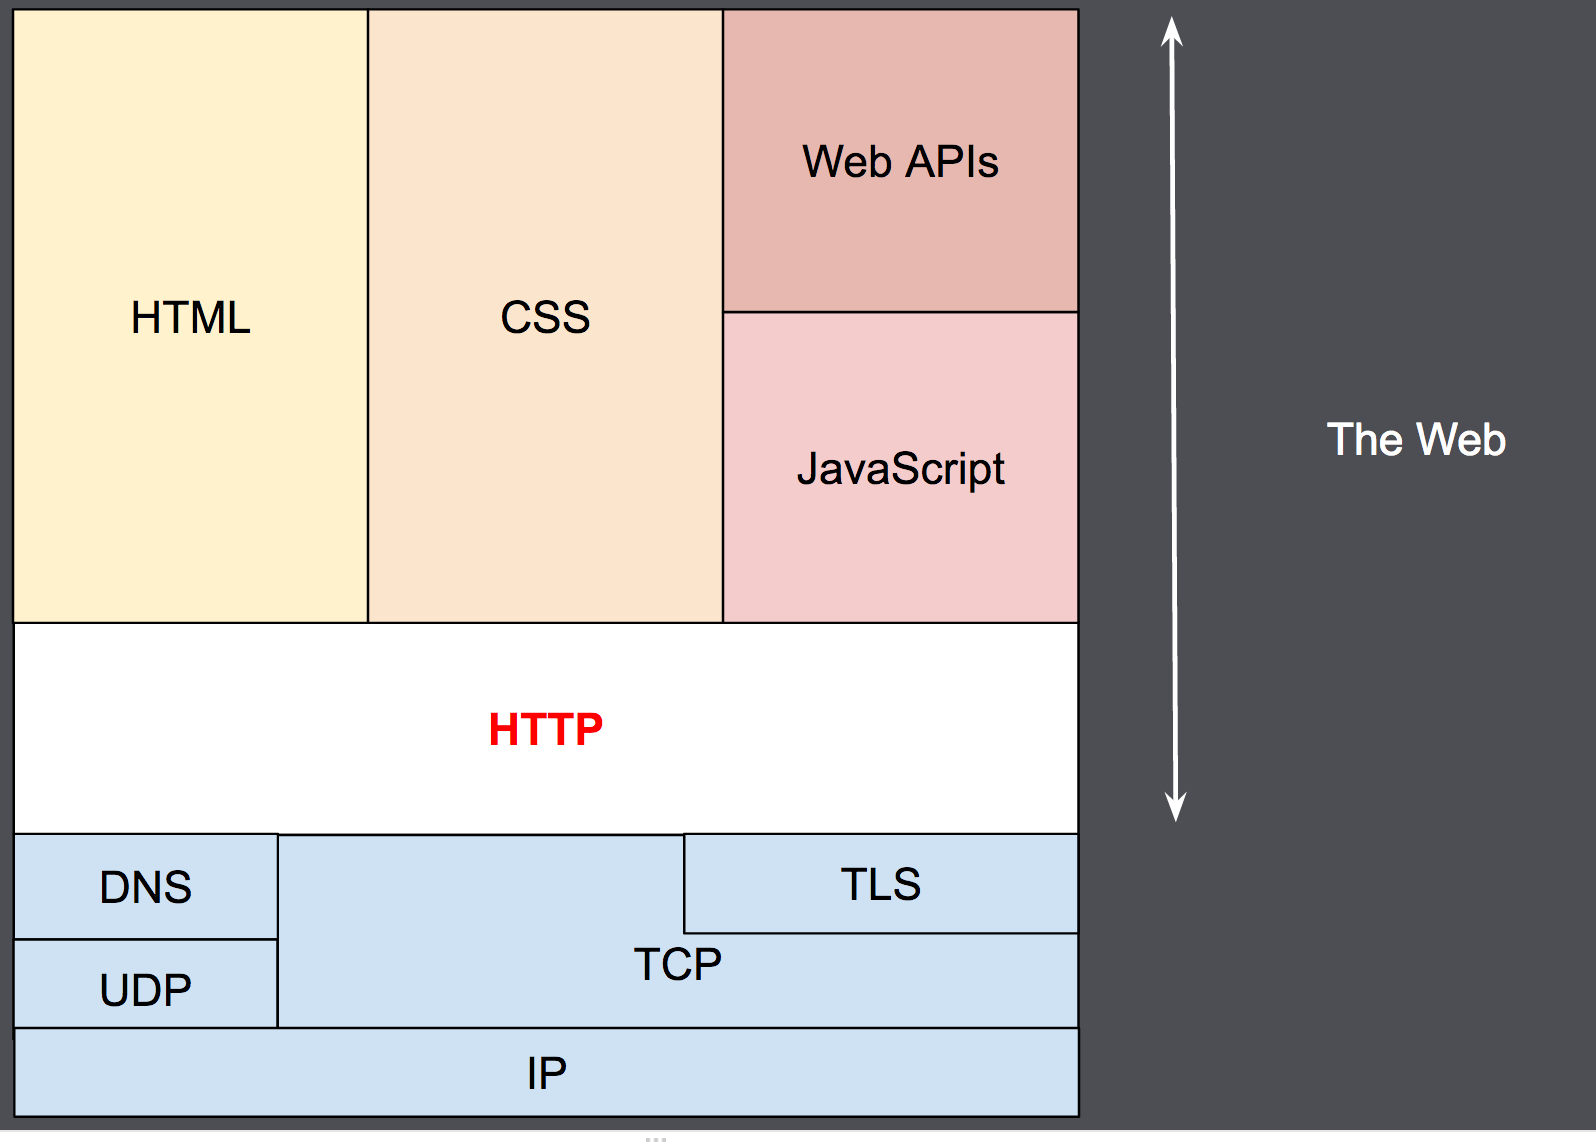
\includegraphics[width=1\textwidth]{HTTPyCapas.png}
	\caption{HTTP y capas}
	\label{fig:super}
\end{figure}

Diseñado a principios de la década de 1990, HTTP es un protocolo ampliable, que ha ido evolucionando con el tiempo. Es lo que se conoce como un protocolo de la capa de aplicación, y se transmite sobre el protocolo TCP, o el protocolo encriptado TLS (en-US), aunque teóricamente podría usarse cualquier otro protocolo fiable. Gracias a que es un protocolo capaz de ampliarse, se usa no solo para transmitir documentos de hipertexto (HTML), si no que además, se usa para transmitir imágenes o vídeos, o enviar datos o contenido a los servidores, como en el caso de los formularios de datos. HTTP puede incluso ser utilizado para transmitir partes de documentos, y actualizar páginas Web en el acto.

En realidad, hay más elementos intermedios, entre un navegador y el servidor que gestiona su petición: hay otros tipos de dispositivos: como routers, modems ... Es gracias a la arquitectura en capas de la Web, que estos intermediarios, son transparentes al navegador y al servidor, ya que HTTP se apoya en los protocolos de red y transporte. HTTP es un protocolo de aplicación, y por tanto se apoya sobre los anteriores. Aunque para diagnosticar problemas en redes de comunicación, las capas inferiores son irrelevantes para la definición del protocolo HTTP . 

\subsection{Características clave del protocolo HTTP}
\begin{itemize}
	\item \textbf{HTTP es sencillo}: HTTP esta pensado y desarrollado para ser leído y fácilmente interpretado por las personas, haciendo de esta manera más facil la depuración de errores, y reduciendo la curva de aprendizaje para las personan que empieza a trabajar con él.
	\item \textbf{HTTP es extensible}: Presentadas en la versión HTTP/1.0, las cabeceras de HTTP, han hecho que este protocolo sea fácil de ampliar y de experimentar con él. Funcionalidades nuevas pueden desarrollarse, sin más que un cliente y su servidor, comprendan la misma semántica sobre las cabeceras de HTTP.
	\item \textbf{HTTP es un protocolo con sesiones, pero sin estados}: HTTP es un protocolo sin estado, es decir: no guarda ningún dato entre dos peticiones en la mísma sesión. Esto crea problemáticas, en caso de que los usuarios requieran interactuar con determinadas páginas Web de forma ordenada y coherente, por ejemplo, para el uso de "cestas de la compra" en páginas que utilizan en comercio electrónico. Pero, mientras HTTP ciertamente es un protocolo sin estado, el uso de HTTP cookies, si permite guardar datos con respecto a la sesión de comunicación. Usando la capacidad de ampliación del protocolo HTTP, las cookies permiten crear un contexto común para cada sesión de comunicación.
	\item \textbf{HTTP y conexiones:} Una conexión se gestiona al nivel de la capa de trasporte, y por tanto queda fuera del alcance del protocolo HTTP. Aún con este factor, HTTP no necesita que el protocolo que lo sustenta mantenga una conexión continua entre los participantes en la comunicación, solamente necesita que sea un protocolo fiable o que no pierda mensajes (como mínimo, en todo caso, un protocolo que sea capaz de detectar que se ha pedido un mensaje y reporte un error). De los dos protocolos más comunes en Internet, TCP es fiable, mientras que UDP, no lo es. Por lo tanto HTTP, se apoya en el uso del protocolo TCP, que está orientado a conexión, aunque una conexión continua no es necesaria siempre. \\
	Todavía hoy se sigue investigando y desarrollando para conseguir un protocolo de transporte más conveniente para el HTTP. Por ejemplo, Google está experimentado con QUIC, que se apoya en el protocolo UDP y presenta mejoras en la fiabilidad y eficiencia de la comunicación. 
\end{itemize}
\subsection{¿Qué se puede controlar con HTTP?}
Se presenta a continuación una lista con los elementos que se pueden controlar con el protocolo HTTP:
\begin{itemize}
	\item \textbf{Cache}: El como se almacenan los documentos en la caché, puede ser especificado por HTTP. El servidor puede indicar a los proxies y clientes, que quiere almacenar y durante cuanto tiempo. Aunque el cliente, también puede indicar a los proxies de caché intermedios que ignoren el documento almacenado.
	\item \textbf{Flexibilidad del requisito de origen} Para prevenir invasiones de la privacidad de los usuarios, los navegadores Web, solamente permiten a páginas del mismo origen, compartir la información o datos. Esto es una complicación para el servidor, asi que mediante cabeceras HTTP, se puede flexibilizar o relajar esta división entre cliente y servidor
	\item \textbf{Autentificación} Hay páginas Web, que pueden estar protegidas, de manera que solo los usuarios autorizados puedan acceder. HTTP provee de servicios básicos de autentificación, por ejemplo mediante el uso de cabeceras como:  WWW-Authenticate, o estableciendo una sesión especifica mediante el uso de  HTTP cookies. 
	\item \textbf{Proxies y  tunneling} Servidores y/o clientes pueden estar en intranets y esconder así su verdadera dirección IP a otros. Las peticiones HTTP utilizan los proxies para acceder a ellos. Pero no todos los proxies son HTTP proxies. El protocolo SOCKS, por ejemplo, opera a un nivel más bajo. Otros protocolos, como el FTP, pueden ser servidos mediante estos proxies.
	\item \textbf{Sesiones} El uso de HTTP cookies permite relacionar peticiones con el estado del servidor. Esto define las sesiones, a pesar de que por definición el protocolo HTTP es un protocolo sin estado. Esto es muy útil no sólo para aplicaciones de comercio electrónico, sino también para cualquier sitio que permita configuración al usuario.
\end{itemize}

\subsection{Mensajes HTTP}
Existen dos tipos de mensajes HTTP: peticiones y respuestas, cada uno sigue su propio formato.

Las peticiones y respuestas HTTP, comparten una estructura similar, compuesta de:

\begin{itemize}
\item Una línea de inicio ('start-line' en inglés) describiendo la petición a ser implementada, o su estado, sea de éxito o fracaso. Esta línea de comienzo, es siempre una única línea.
\item Un grupo opcional de cabeceras HTTP, indicando la petición o describiendo el cuerpo ('body' en inglés) que se incluye en el mensaje. 
\item Una línea vacía ('empty-line' en inglés) indicando toda la meta-información ha sido enviada.
\item Un campo de cuerpo de mensaje opcional ('body' en inglés) que lleva los datos asociados con la petición (como contenido de un formulario HTML), o los archivos o documentos asociados a una respuesta (como una página HTML, o un archivo de audio, vídeo ... ) . La presencia del cuerpo y su tamaño es indicada en la línea de inicio y las cabeceras HTTP.

\end{itemize}
La línea de inicio y las cabeceras HTTP, del mensaje, son conocidas como la cabeza de la peticiones, mientras que su contenido en datos se conoce como el cuerpo del mensaje.

\begin{figure}[H]
	\center
	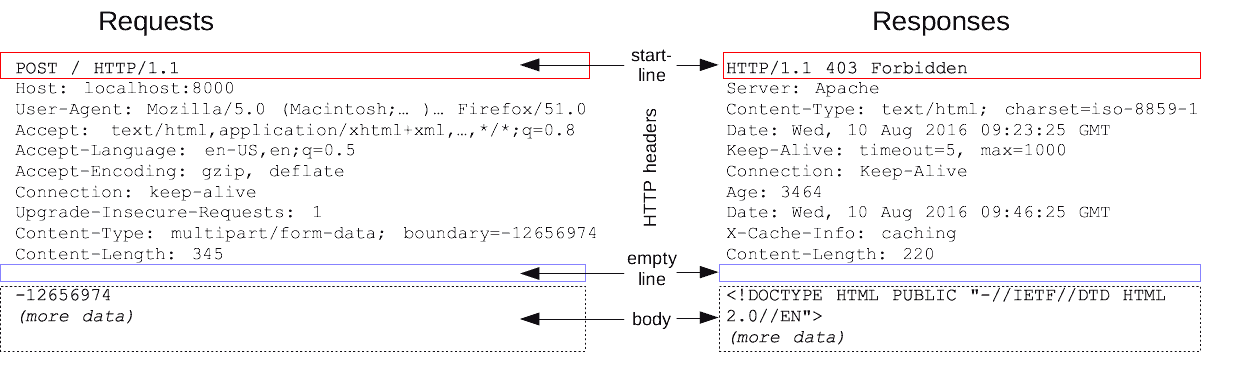
\includegraphics[width=0.7\textwidth]{HTTPMsgStructure2.png}
	\caption{Mensajes}
	\label{fig:super}
\end{figure}

\subsubsection{Cabeceras}

Las cabeceras HTTP  de una petición siguen la misma estructura que la de una cabecera HTTP. Una cadena de caracteres, que no diferencia mayusculas ni minusculas, seguida por dos puntos  (':')  y un valor cuya estructura depende de la cabecera. La cabecera completa, incluido el valor, ha de ser formada en una única línea, y pude ser bastante larga. 

Hay bastantes cabeceras posibles. Estas se pueden clasificar en varios grupos: 
\begin{itemize}
	\item Cabeceras generales, ('General headers' en inglés), como Via (en-US),  afectan al mensaje como una unidad completa.
	\item Cabeceras de petición, ('Request headers' en inglés), como User-Agent, Accept-Type, modifican la petición especificándola en mayor detalle ( como: Accept-Language (en-US), o dándole un contexto, como:  Referer, o restringiéndola condicionalmente, como: If-None.
	\item Cabeceras de entidad, ('Entity headers' en ingles), como Content-Length las cuales se aplican al cuerpo de la petición. Por supuesto, esta cabecera no necesita ser transmitida si el mensaje no tiene cuerpo ('body' en inglés). 
\end{itemize}

\begin{figure}[H]
	\center
	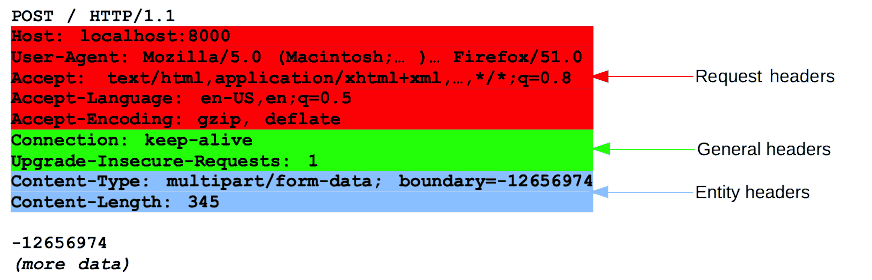
\includegraphics[width=0.7\textwidth]{HTTP_Request_Headers2.png}
	\caption{Cabeceras}
	\label{fig:super}
\end{figure}

\subsubsection{Cuerpo}
La parte final de la petición el el cuerpo. No todas las peticiones llevan uno: las peticiones que reclaman datos, como GET, HEAD, DELETE, o OPTIONS, normalmente, no necesitan ningún cuerpo. Algunas peticiones pueden mandar peticiones al servidor con el fin de actualizarlo: como es el caso con la petición POST  (que contiene datos de un formulario HTML). 
\\
Los cuerpos pueden ser dividos en dos categorias:
\begin{itemize}
	\item Cuerpos con un único dato, que consisten en un único archivo defindo por las dos cabeceras: Content-Type y Content-Length.  
	\item Cuerpos con múltiples datos, que están formados por distintos contenidos, normalmente estan asociados con los formularios HTML. 
\end{itemize}

\subsubsection{Peticiones}
Un ejemplo de petición HTTP:

\begin{figure}[H]
	\center
	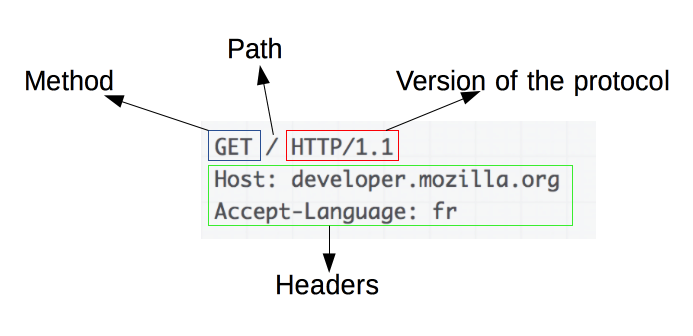
\includegraphics[width=0.7\textwidth]{HTTP_Request.png}
	\caption{Petición}
	\label{fig:super}
\end{figure}
Una petición de HTTP, está formado  por los siguientes campos:

\begin{itemize}
	\item Un método HTTP,  normalmente pueden ser un verbo, como: GET, POST o un nombre como: OPTIONS (en-US) o HEAD (en-US), que defina la operación que el cliente quiera realizar. El objetivo de un cliente, suele ser una petición de recursos, usando GET, o presentar un valor de un formulario HTML, usando POST, aunque en otras ocasiones puede hacer otros tipos de peticiones. 
	\item La dirección del recurso pedido; la URL del recurso, sin los elementos obvios por el contexto, como pueden ser: sin el  protocolo (http://),  el dominio (aquí developer.mozilla.org), o el puerto TCP (aquí el 80). 
	\item La versión del protocolo HTTP.
	\item Cabeceras HTTP opcionales, que pueden aportar información adicional a los servidores.
	\item O un cuerpo de mensaje, en algún método, como puede ser POST, en el cual envía la información para el servidor.
\end{itemize}

\subsubsection{Respuestas}
Un ejemplo de repuesta:
\begin{figure}[H]
	\center
	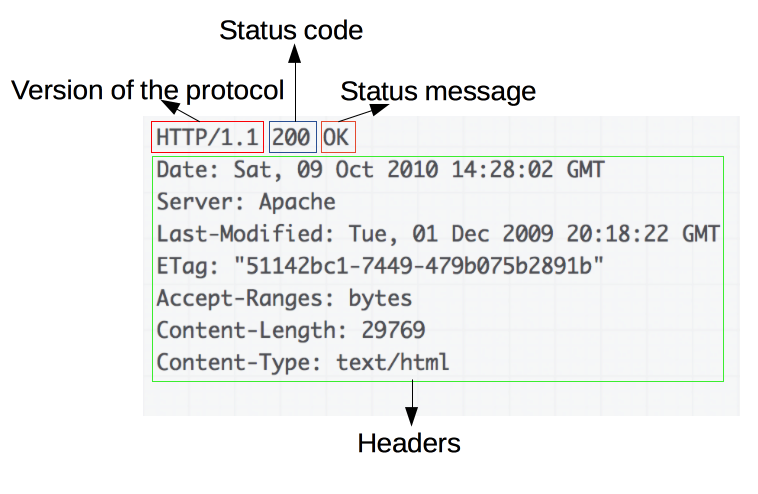
\includegraphics[width=0.7\textwidth]{HTTP_Response.png}
	\caption{Respuesta}
	\label{fig:super}
\end{figure}
Las respuestas están formadas por los siguentes campos:

\begin{itemize}
	\item La versión del protocolo HTTP que están usando.
	\item Un código de estado, indicando si la petición ha sido exitosa, o no, y debido a que. Códigos de estado muy comunes son:  200, 404, o 302
	\item Un mensaje de estado, una breve descripción del código de estado. 
	\item Cabeceras HTTP, como las de las peticiones.
	\item Opcionalmente, el recurso que se ha pedido.
\end{itemize}

\subsection{Métodos de petición HTTP}

HTTP define un conjunto de métodos de petición para indicar la acción que se desea realizar para un recurso determinado. Aunque estos también pueden ser sustantivos, estos métodos de solicitud a veces son llamados HTTP verbs. Cada uno de ellos implementan una semántica diferente, pero algunas características similares son compartidas por un grupo de ellos: ej. un request method puede ser safe, idempotent (en-US), o cacheable.

\subsubsection{GET}
El método GET  solicita una representación de un recurso específico. Las peticiones que usan el método GET sólo deben recuperar datos.

\begin{figure}[H]
	\center
	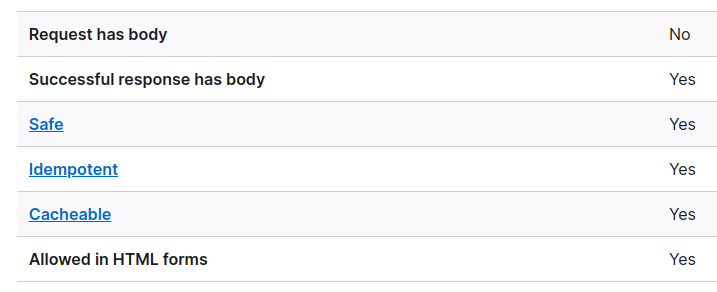
\includegraphics[width=0.7\textwidth]{get.png}
	\caption{GET}
	\label{fig:super}
\end{figure}

\subsubsection{HEAD}
El método HEAD pide una respuesta idéntica a la de una petición GET, pero sin el cuerpo de la respuesta.

\subsubsection{POST}
El método POST se utiliza para enviar una entidad a un recurso en específico, causando a menudo un cambio en el estado o efectos secundarios en el servidor. \\
El tipo de cuerpo de la solicitud se indica mediante el encabezado Content-Type.

\begin{figure}[H]
	\center
	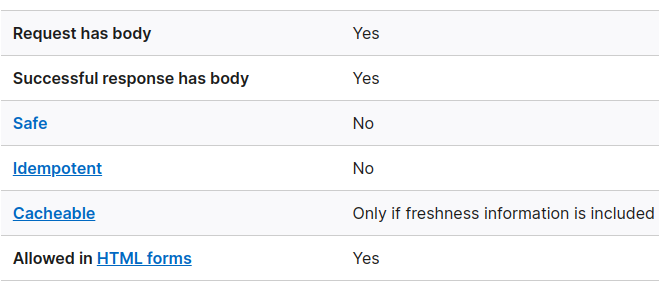
\includegraphics[width=0.7\textwidth]{post.png}
	\caption{POST}
	\label{fig:super}
\end{figure}

\subsection{Status}
\subsection{URI - URL}
\subsection{Headers}

\section{Modelo de Objetos de Documento - DOM}

\section{Gestor de contenidos}

\section{REST}

\section{Entorno de desarrollo}

nodejs
https://github.com/nodesource/distributions/blob/master/README.md

Angular: npm install -g @angular/cli

Set-ExecutionPolicy RemoteSigned -Scope CurrentUser
get-ExecutionPolicy -list

\section{Backend}
\subsection{Postman - Thunder client - curl}
\subsection{Frameworks}
\subsection{Java}
\subsection{Spring boot}
\subsection{Spring data}
\subsection{Postgres - Mongo - Elastic Search}
\subsection{CRUD}
\subsubsection{Entidades - DTOs}
\subsubsection{Repositorios}
\subsubsection{Servicios}
\subsubsection{Controladores}

\section{Frontend}
\subsection{Frameworks}
\subsection{Angular}
\subsection{HTML}
\subsection{CSS}
\subsubsection{Frameworks CSS}
\subsubsection{Tailwind CSS}
\subsection{Javascript - ECMAScript}
\subsection{Typescript}
\subsection{CRUD}
\subsubsection{Entidades - DTOs}
\subsubsection{Servicios}
\subsubsection{Componentes}
\subsubsection{Input - Output}
\subsection{Temas}
\subsection{Menús}
\section{Ramificación GIT}